\section{Preliminaries: Bernoulli percolation on hierarchical lattices}\label{sec:bernoulli}

在这一节中，我们给出经典 EIGS 层级晶格上 Bernoulli 渗流的基本性质，作为后文研究的基础。

第~\ref{sec:percolation-preliminaries} 小节主要研究非平凡贯通相变的存在性，以及如何将临界端点团簇表示为 random EIGS。这一部分既包含对 Hambly 和 Kumagai~\cite{hambly2010diffusion} 的构造的推广，也有与 Alves、Baldasso、Moreira 和 Teixeira~\cite{alves2026percolation} 最近的工作重叠的内容。
为了文章的连贯性，我们仍然列出这些结果，同时明确标注它们与已有文献的关系。

第~\ref{sec:live-matrix} 小节讨论由渗流导出的 random EIGS 的质量转移矩阵及其谱结构。
这些性质是理解临界团簇及其临界指数的重要基础。


%%%%%%%%%%%%%%%%%%%%%%%%%%%%%%%%%%%%%%
\subsection{From percolation to random EIGS}\label{sec:percolation-preliminaries}

在欧氏晶格上，Bernoulli 渗流通常难以精确求解；
而在经典 EIGS 层级晶格上，精确重整化给出了研究贯通概率和端点团簇的递归方法。
更进一步，在临界点并以两端点连通为条件，端点团簇可以由一个 random EIGS 表示，我们因而可以通过研究这个 random EIGS 来理解团簇的性质。

\begin{definition}\label{def:bernoulli}
On each substitution graph $\Xi^n$, a configuration is a subset $\omega\subseteq E(\Xi^n)$ of open edges. Under $\mathbb P_p$, these edges are independently open with probability $p\in[0,1]$, so a particular configuration has probability $p^{|\omega|}(1-p)^{|E(\Xi^n)|-|\omega|}$. Its clusters are the connected components of the graph with vertex set $V(\Xi^n)$ and edge set $\omega$, including isolated vertices. The inherited terminals are denoted by $\mathfrak v_+,\mathfrak v_-$.

For a finite two-terminal graph $G$, its reliability is
\[
 \varphi_G(p):=\mathbb P_p(\text{the terminals of }G\text{ are connected}).
\]
\end{definition}
Summing the configuration probabilities over the connecting edge subsets makes $\varphi_G$ an integer polynomial. We study the terminal crossing transition and the conditional clusters seen from the terminals. The finite graphs need not form a nested sequence of edge sets; replacing an edge removes it and inserts a new cell.



\begin{lemma}[Also see \cite{alves2026percolation}]\label{lem:renormalisation}
For every $n\ge 1$ and every $p\in[0,1]$,
\[
    \varphi_{\Xi^{n}:\mathfrak v_+\leftrightarrow \mathfrak v_-}(p)
    =
    \varphi_{R:\beta^+\leftrightarrow \beta^-}^{\circ n}(p),
\]
where $\varphi_R^{\circ n}$ denotes the $n$-fold composition of $\varphi_R$ with itself.
\end{lemma}
\begin{proof}
By construction $\Xi^{n}$ is obtained from the rule graph $R$ by substituting a fresh copy of $\Xi^{n-1}$ for each of its edges, the copies being glued only at the planting vertices.
Distinct copies share no edge, so under $\mathbb P_p$ their percolation configurations are independent, and each copy connects the two planting vertices of the edge it replaces with probability $\varphi_{\Xi^{n-1}}(p)$.

The crossing event $\{\mathfrak v_+\leftrightarrow\mathfrak v_-\}$ in $\Xi^{n}$ depends on the percolation configuration only through the family of crossing events of the substituted copies, one per edge of $R$.
These indicators are independent and each has mean $\varphi_{\Xi^{n-1}}(p)$, and the global crossing occurs precisely when the corresponding edges of $R$ form a crossing of $R$.
Hence the crossing of $\Xi^{n}$ has the law of the crossing of $R$ with independent edge-occupation $\varphi_{\Xi^{n-1}}(p)$, which gives
\[
    \varphi_{\Xi^{n}}(p)=\varphi_{R}\bigl(\varphi_{\Xi^{n-1}}(p)\bigr).
\]

For $n=1$ the substitution replaces the single initial edge by one copy of $R$, so $\varphi_{\Xi^{1}}=\varphi_R$.
Iterating the displayed recursion and using $\varphi_{\Xi^{1}}=\varphi_R$ yields $\varphi_{\Xi^{n}}=\varphi_R^{\circ n}$.
\end{proof}



\begin{proposition}[Also see \cite{alves2026percolation}]\label{prop:nontrivial-transition}
For a finite connected two-terminal rule graph $R$, the function $\varphi_R(p)-p$ changes sign in $(0,1)$ if and only if
\[
 \dist_R(\beta^+,\beta^-)\ge2,
 \qquad \lambda_R(\beta^+,\beta^-)\ge2.
\]
\end{proposition}
\begin{proof}
If the terminal distance is at least two, a union bound over the finitely many simple terminal paths gives $\varphi_R(p)=O(p^2)$ as $p\downarrow0$.
If the minimum terminal cut has at least two edges, a union bound over the finitely many terminal cuts gives $1-\varphi_R(p)=O((1-p)^2)$ as $p\uparrow1$.
Thus $\varphi_R(p)<p$ near zero and $\varphi_R(p)>p$ near one.
Continuity gives an interior sign change.

Conversely, if the terminals are adjacent, opening a direct edge suffices for connection, so $\varphi_R(p)\ge p$ throughout $[0,1]$.
If the minimum terminal cut has size one, its unique edge must be open for connection, so $\varphi_R(p)\le p$ throughout $[0,1]$.
Neither case permits a sign change.
\end{proof}

This criterion does not require canonicality or terminal symmetry; see also~\cite{alves2026percolation}*{Remark~5}.
When the terminal distance is at least two and the minimum cut has size one, the latter inequality is strict for $0<p<1$: opening only the separating edge does not connect the terminals.
Consequently $\displaystyle\lim_{n\to\infty}\varphi_R^{\circ n}(p)=0$ for every $p<1$.
The condition $\lambda_R(\beta^+,\beta^-)\ge2$ therefore excludes precisely this trivial crossing regime once $\ell\ge2$.
Under the two geometric bounds, the following theorem gives uniqueness and strict instability of the interior fixed point, as also established in~\cite{alves2026percolation}*{Theorem~3.1}.

\begin{theorem}[Also see \cite{alves2026percolation}]
\label{thm:unique-unstable-critical-point}
For a finite connected two-terminal rule graph with terminal distance at least two and minimum terminal edge cut at least two, the reliability function $\varphi_R$ has a unique fixed point $p_c\in(0,1)$, and this fixed point is unstable:
\[
    \varphi_R'(p_c)>1.
\]
\end{theorem}

\begin{proof}
For $p\in(0,1)$, Russo's formula and the Bernoulli Poincar\'e inequality give $\varphi_R(p)(1-\varphi_R(p))\le p(1-p)\varphi_R'(p)$. Equality in the Poincar\'e inequality forces every term of degree at least two in the $p$-biased Walsh expansion to vanish, so a monotone Boolean function attaining equality is constant or depends on a single coordinate. The crossing indicator is nonconstant and, since the terminal distance is at least two, cannot be determined by a single edge, so the inequality is strict. Consequently, $\log\frac{\varphi_R(p)}{1-\varphi_R(p)}-\log\frac{p}{1-p}$ is strictly increasing on $(0,1)$. Union bounds over terminal paths and separating cuts give $\varphi_R(p)=O(p^{\ell_R})$ as $p\downarrow0$ and $1-\varphi_R(p)=O((1-p)^{\lambda_R(\beta^+,\beta^-)})$ as $p\uparrow1$. Since both geometric exponents are at least two, this log-odds difference tends to $-\infty$ at zero and to $+\infty$ at one. It therefore has exactly one zero $p_c\in(0,1)$, equivalently $\varphi_R(p_c)=p_c$. Evaluating the strict inequality at $p_c$ and dividing by $p_c(1-p_c)$ yields $\varphi_R'(p_c)>1$.
\end{proof}


\begin{corollary}[Also see \cite{alves2026percolation}]
\label{cor:global-renormalisation-dichotomy}
Under the assumptions of Theorem~\ref{thm:unique-unstable-critical-point},
the unique critical fixed point \(p_c\in(0,1)\) separates the renormalisation
flow:
\[
    \varphi_R(p)<p
    \quad\text{for }0<p<p_c,
    \qquad
    \varphi_R(p)>p
    \quad\text{for }p_c<p<1.
\]
Consequently,
\[
    \displaystyle\lim_{n\to\infty}\varphi_R^{\circ n}(p)
    =
    \begin{cases}
        0, & 0\le p<p_c,\\[2mm]
        p_c, & p=p_c,\\[2mm]
        1, & p_c<p\le 1.
    \end{cases}
\]
\end{corollary}



\begin{corollary}[Also see \cite{alves2026percolation}]
\label{cor:iterated-linearisation}
Let \(p_c\) be the unique fixed point of \(\varphi_R\) in \((0,1)\).
Then, for every \(n\ge 1\),
\[
    \left(\varphi_R^{\circ n}\right)'(p_c)
    =
    \varphi_R'(p_c)^n.
\]
In particular, since \(\varphi_R'(p_c)>1\) by Theorem~\ref{thm:unique-unstable-critical-point}, the fixed point \(p_c\) is exponentially
repelling under the renormalisation flow.
\end{corollary}




\begin{example}\label{ex:dhl-reliability}
For DHL,
\[
 \varphi_R(p)=1-(1-p^2)^2=2p^2-p^4,\qquad
 p_c=\frac{\sqrt5-1}{2},\qquad
 \varphi_R'(p_c)=4p_c(1-p_c^2)=6-2\sqrt5.
\]
The fixed point therefore has a strictly expanding pivotal response, although the probability of crossing a cell is unchanged there.
\end{example}

\begin{figure}[tbp]
\centering
\begin{minipage}[c]{0.40\textwidth}
\centering
\begin{tikzpicture}[scale=1.0,vertex/.style={circle,fill=black,inner sep=1.7pt}]
\draw (0,0)--(0.8,0);
\node[vertex] at (0,0) {};\node[vertex] at (0.8,0) {};
\draw[-{Stealth}] (1.05,0)--(1.7,0);
\draw (2,0)--(3,0.8)--(4,0)--(3,-0.8)--cycle;
\foreach \x/\y in {2/0,3/0.8,4/0,3/-0.8}{\node[vertex] at (\x,\y) {};}
\node[below left] at (2,0) {$\beta^+$};
\node[below right] at (4,0) {$\beta^-$};
\end{tikzpicture}
\end{minipage}\hfill
\begin{minipage}[c]{0.55\textwidth}
\centering
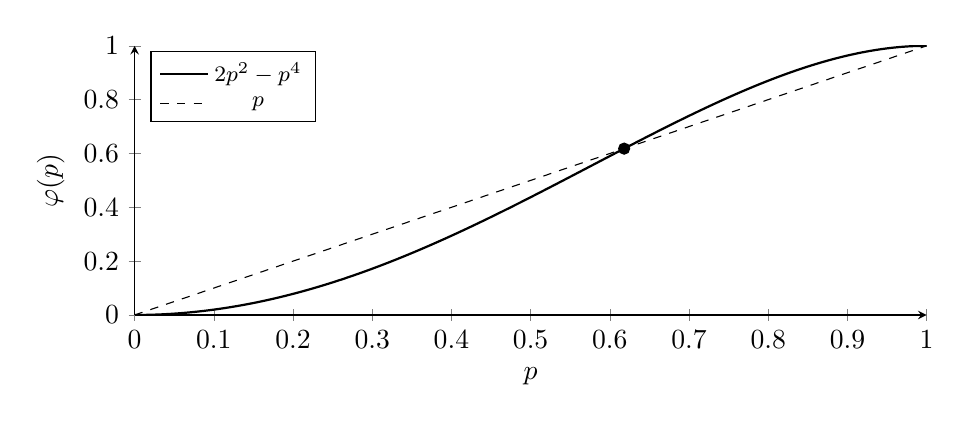
\begin{tikzpicture}
\begin{axis}[width=0.96\textwidth,height=5cm,xmin=0,xmax=1,ymin=0,ymax=1,
axis lines=left,xlabel={$p$},ylabel={$\varphi(p)$},samples=160,
legend style={font=\footnotesize,at={(0.02,0.98)},anchor=north west}]
\addplot[thick,domain=0:1] {2*x^2-x^4};\addlegendentry{$2p^2-p^4$}
\addplot[dashed,domain=0:1] {x};\addlegendentry{$p$}
\addplot[only marks,mark=*] coordinates {(0.6180339887,0.6180339887)};
\end{axis}
\end{tikzpicture}
\end{minipage}
\caption{The diamond substitution rule and its reliability map. The marked interior intersection with the diagonal is $p_c=(\sqrt5-1)/2$. The substitution arrow does not orient the graph edges.}
\label{fig:dhl-reliability}
\end{figure}














%%%%%%%%%%%%%%%%%%%%%%%%%%%%%%%%%%%%%%%%%%%%%%%%%%%%%%%%%%%%%%%%%%%%%

Hambly and Kumagai~\cite{hambly2010diffusion} described the critical two-terminal cluster on the diamond lattice through a finite-type random recursive construction and its geometric limit.
We formulate this construction in the language of random EIGS and extend it to every classical EIGS hierarchical lattice.
The random EIGS specifies the recursive generating mechanism, and its finite approximations are random substitution networks. Under a compatible contractive realisation, its geometric limit is a graph-directed random recursive fractal.
The auxiliary types record which terminals of a cell belong to the cluster being followed; they are needed even though the final cluster consists only of open edges.

Let $A^+$ and $A^-$ be the open clusters of the two terminals inside a rule cell.
A parent of state $c$ uses the event $\beta^+\leftrightarrow\beta^-$ and its common terminal cluster as the active set.
A parent of state $b$ uses the complementary event and active set $A^+\cup A^-$.
A parent of state $u$ uses the complementary event and active set $A^+$.
Terminal symmetry makes the corresponding one-terminal expectations independent of which terminal is chosen.
For a union $A$ of active open clusters, the child state of $e=\{x,y\}$ is
\[
 \operatorname{st}_{A,\omega}(e):=
 \begin{cases}
 c,&x,y\in A\text{ and }e\text{ is open},\\
 b,&x,y\in A\text{ and }e\text{ is closed},\\
 u,&\text{exactly one of }x,y\text{ lies in }A,\\
 0,&x,y\notin A.
 \end{cases}
\]
An edge in state $u$ is necessarily closed.
The state $0$ records no active endpoint and produces no live descendant under refinement.


\begin{definition}\label{def:random-eigs}
Fix $p\in(0,1)$ and a live parent state $\sigma\in\{c,b,u\}$. Sample a Bernoulli configuration with parameter $p$ in its rule cell conditioned on the parent event just specified, and label every child edge by its active state. Repeat this operation inside the live children, with independent conditional samples for distinct child cells once their parent states are fixed. A state-$0$ cell has no live descendants. For a state-$u$ child its active terminal is inherited from the parent; terminal symmetry identifies the two possible orientations in distribution.
\end{definition}

To obtain a geometric limit from edge-substitution rules, we first specify a compatible realisation by contractions.
In the graph-directed construction of Hambly and Kumagai~\cite{hambly2010diffusion}*{Section~3.2}, vertices of the construction graph play the role of edge colours in the EIGS.
A \emph{compatible contractive realisation} requires the initial graph and all rule graphs to have no isolated vertices, and assigns to each colour $i$ a nonempty compact metric space $X_i$ with two distinct marked terminals.
For each rule of colour $i$, its vertices are placed injectively in $X_i$, with its planting vertices at these terminals.
Each rule edge $e$ of colour $j$ is represented by an injective contraction $\psi_e:X_j\longrightarrow X_i$ sending the ordered terminals to the endpoints of $e$.
Images of distinct child spaces intersect exactly at the prescribed common endpoints, and all maps have Lipschitz constants at most a common $q<1$.
The maps retain their parent colour and rule as part of their indexing.
Thus the realisation retains both the graph incidence data and the rule laws of Definition~\ref{definition:EIGS}.

\begin{theorem}\label{thm:eigs-graph-directed}
The geometric limit of every (random) EIGS with a compatible contractive realisation is a graph-directed (random) recursive fractal, with edge colours as vertex types.
\end{theorem}
\begin{proof}
It suffices to start from one edge of colour $i$; a finite initial graph is obtained by the prescribed terminal identifications of finitely many such constructions.
Make one construction-graph vertex for each colour.
For each rule of colour $i$ and each of its edges $e$ of colour $j$, introduce a directed edge from $i$ to $j$, carrying $\psi_e$ and its endpoint incidence data.
Edges arising from different rules are kept distinct.
At a cell of type $i$, select the entire outgoing family belonging to one rule with precisely that rule's probability.
Do this independently in different cells.
In particular, children of one cell are not sampled independently of one another.
This is the finite-type graph-directed random recursive construction: the construction graph records types, while its maps and incidence data specify the geometric copies and their gluing.

Couple the two descriptions by using the same rule choice at every cell.
Their root types agree.
Whenever their depth-$n$ cells agree, the common rule choices give identical child types, contractions and endpoint identifications.
Induction identifies all finite-level labelled cell structures, and hence their joint laws, including the realised substitution graphs.

For a fixed realisation $\omega$, let $T_n(i,\omega)$ be the depth-$n$ cell addresses issued from type $i$, let $i(w)$ be the colour at address $w$, and let $\psi_w$ be the composition of the maps along $w$.
The finite unions
\[
 \bigcup_{w\in T_n(i,\omega)}\psi_w(X_{i(w)})
\]
are nonempty compact subsets of $X_i$ and decrease with $n$.
Their intersection therefore defines a nonempty compact set
\[
 K_i(\omega):=
 \bigcap_{n\ge0}\ \bigcup_{w\in T_n(i,\omega)}
       \psi_w(X_{i(w)}).
\]
Every depth-$n$ cell has diameter at most $q^n\max_j\operatorname{diam}(X_j)$.
Each infinite address consequently determines a unique point, and every point of $K_i(\omega)$ has such an address, by finite branching and nestedness.
Writing $R_i(\omega)$ for the first rule and $\omega_e$ for the subsequent choices below its edge $e$, we obtain
\[
 K_i(\omega)=
 \bigcup_{e\in E(R_i(\omega))}
       \psi_e\bigl(K_{\operatorname{col}(e)}(\omega_e)\bigr),
\]
where $\operatorname{col}(e)$ denotes the edge colour.
This is the graph-directed random recursive set equation.

The compatibility conditions also identify this set with the geometric limit of the EIGS.
Indeed, every vertex in a realised substitution graph remains a vertex at all subsequent levels.
Every depth-$n$ cell contains its two terminal vertices, so, if $V_i^n(\omega)$ is the realised level-$n$ vertex set,
\[
 d_{\mathrm{Haus}}^{X_i}
       \bigl(V_i^n(\omega),K_i(\omega)\bigr)
 \le q^n\max_j\operatorname{diam}(X_j).
\]
Here each finite-level vertex belongs to the intersection, and each point of the intersection lies within the stated diameter of a terminal of a depth-$n$ cell.
Thus the graph-directed attractor is the geometric limit of the realised EIGS, and the two recursive descriptions agree pathwise at every finite level.
The generating EIGS can be recovered from the graph-directed description when the rule families, probabilities and two-terminal incidence data are retained; the attractor alone does not specify these data.
The deterministic case is obtained by taking point-mass rule laws.
\end{proof}

For $n\ge0$, let $\mathfrak C_n$ denote the common open cluster of the two terminals in $\Xi^n$, under critical Bernoulli percolation conditioned on their connection.
The cluster includes all open branches attached to the terminals, not only edges lying on an open terminal-to-terminal path.
The labels $b,u,0$ are auxiliary states; the state-$c$ edges form the open subgraph extracted from the random EIGS.

\begin{theorem}[Generalisation of the Hambly--Kumagai theorem~\cite{hambly2010diffusion}]\label{thm:percolation-random-eigs}
On every classical EIGS hierarchical lattice, critical Bernoulli bond percolation conditioned on terminal connection induces a random EIGS representation of its cluster.
\end{theorem}
\begin{proof}
Fix a finite depth and coarsen each bottom-level cell to an open edge precisely when its two terminals are connected inside that cell.
The cells have disjoint edge sets, so their crossing indicators are independent.
Each indicator has probability $\varphi_R(p_c)=p_c$.
Repeating the coarsening therefore gives the critical Bernoulli law at every level.

Conditioning on the full coarse configuration fixes whether each child cell connects its terminals.
The configurations in distinct child cells remain independent under these individual conditions, since the original edge sets are disjoint.
Within a connected cell, the active part is its common terminal cluster.
Within a disconnected cell, the active part is the union of its two terminal clusters, one specified terminal cluster, or neither, according to the active endpoints inherited from the parent.
These are exactly the conditional laws for $c,b,u,0$ in Definition~\ref{def:random-eigs}.
For a one-terminal cell, the active endpoint is retained; terminal symmetry permits its identification with the reference orientation used for state $u$.
Offspring labels within one cell may be dependent, as specified by the sampled configuration.

Starting with the root conditioned to connect, induction on the depth now identifies the joint laws of all labelled cells.
At the last level, an open edge belongs to the root cluster exactly when it has state $c$.
Extracting these edges proves the assertion about $\mathfrak C_n$.
\end{proof}

The fixed-point identity is essential to stationarity of this representation.
For a general parameter $p$, the analogous finite-depth construction uses the successive effective probabilities $\varphi_R^{\circ k}(p)$ and hence level-dependent replacement laws.



%%%%%%%%%%%%%%%%%%%%%%%%%%%%%%%%%%%%%%%%%%%%%%%%%%%

The mass transfer matrix of the random EIGS records the expected numbers of live child edges of each type.
Terminal symmetry combines the two oriented one-terminal types into the single state $u$, leaving the three states $c,b,u$.
The matrix and expected-mass results below use only the finite-level representation.


\begin{definition}\label{def:live-matrix}
For $p\in(0,1)$, $\mathbf M_{\mathfrak C}(p)$ is the matrix whose entry $M_{\sigma,\tau}(p)$ is the expected number of state-$\tau$ child edges under the conditional parent law of state $\sigma$, with rows and columns ordered as $(c,b,u)$.
At criticality, we write $\mathbf M_{\mathfrak C}:=\mathbf M_{\mathfrak C}(p_c)$ and denote its spectral radius by $\rho(\mathbf M_{\mathfrak C})$.
All entries refer to the conditional live-state matrix, including when we later pass to an invariant two-dimensional block.
\end{definition}

\begin{proposition}\label{prop:live-matrix-primitive}
For every admissible rule graph and every $p\in(0,1)$, the three-state live matrix $\mathbf M_{\mathfrak C}(p)$ is primitive.
\end{proposition}

\begin{proof}
The rule graph has no bridge.
Indeed, by canonicality a bridge belongs to a simple terminal-to-terminal path, and its deletion would therefore separate the terminals, contrary to the terminal edge-connectivity assumption.
Opening every edge except one consequently gives a connected parent cell containing a child of state $b$, so $M_{c,b}(p)>0$.
Closing every edge gives a disconnected parent cell whose active set for state $b$ consists of the two terminals.
Since the terminals are not adjacent, an edge incident to either terminal then has state $u$, so $M_{b,u}(p)>0$.
Opening exactly one edge incident to $\beta^+$ leaves the terminals disconnected and gives a child of state $c$ in a parent of state $u$, so $M_{u,c}(p)>0$.
These entries give the directed cycle $c\to b\to u\to c$.
The all-open configuration gives $M_{c,c}(p)>0$, so this irreducible matrix is aperiodic and therefore primitive.
\end{proof}

\begin{definition}\label{def:critical-mass-dimension}
The expected critical mass dimension is, when the limit exists,
\[
 \dimmass(\mathfrak C):=\lim_{n\to\infty}
 \frac{\log\mathbb E[|E(\mathfrak C_n)|]}{\log\ell^n},
\]
where the expectation is under critical percolation conditioned on terminal connection.
\end{definition}
This is an expected growth exponent; its identification with an almost-sure Hausdorff dimension of a random scaling limit is a further geometric statement.

\begin{lemma}[Also see \cite{alves2026percolation}]\label{thm:mass-transfer-power}
At $p=p_c$, for every $n\ge1$ and all live states $\sigma,\tau\in\{c,b,u\}$, the expected number of state-$\tau$ live edges of $\Xi^{n}$ contained in a level-zero block of state $\sigma$ equals the $(\sigma,\tau)$ entry of $\bigl(\mathbf M_{\mathfrak C}(p_c)\bigr)^{n}$.
\end{lemma}

\begin{proof}
The case $n=1$ is the definition of the live matrix, since at the critical point the edge occupation entering a single substitution cell is $p_c$.

Replacing every edge of $\Xi^{n}$ by a rule cell at occupation $p_c$ turns each cell into a coarse edge that is open with probability $\varphi_R(p_c)=p_c$, so every level of the substitution sees the same edge occupation $p_c$.
Conditionally on the states of the level-$n$ edges, the configurations of the cells refining distinct edges are independent, and the conditional law inside a cell of coarse state $\tau'$ is the conditioned percolation law defining the row $\tau'$ of the live matrix.
Hence the expected state counts at level $n+1$ inside a state-$\sigma$ block are obtained from those at level $n$ by one application of $\mathbf M_{\mathfrak C}(p_c)$ on the right, and the claim follows by induction.
\end{proof}


\begin{theorem}[Also see \cite{alves2026percolation}]\label{thm:critical-mass-dimension}
For every classical EIGS hierarchical lattice, the expected critical mass dimension exists and
\[
 \dimmass(\mathfrak C)=\frac{\log\rho(\mathbf M_{\mathfrak C})}{\log\ell}.
\]
\end{theorem}
\begin{proof}
By Theorem~\ref{thm:percolation-random-eigs}, the edges of $\mathfrak C_n$ are exactly the state-$c$ edges in the random representation started from state $c$.
Lemma~\ref{thm:mass-transfer-power} therefore gives
\[
 \mathbb E[|E(\mathfrak C_n)|]
 =\bigl(\mathbf M_{\mathfrak C}(p_c)^n\bigr)_{c,c}.
\]
The matrix is primitive by Proposition~\ref{prop:live-matrix-primitive}.
The Perron--Frobenius theorem implies that the right-hand side is $C\rho(\mathbf M_{\mathfrak C})^{\,n}(1+o(1))$ for a constant $C>0$.
Taking logarithms and dividing by $n\log\ell$ proves the formula.
\end{proof}

The total expected number of live cells has the same exponent, because every entry of the Perron projection is positive.
Counting actual open cluster edges or all live cells thus gives the same logarithmic growth rate, although the finite-stage expectations differ.












%%%%%%%%%%%%%%%%%%%%%%%%%%%%%%%%%%%%%%%%%%%%%%%%%%%%%
\subsection{Spectral structure of the mass matrix}\label{sec:live-matrix}

在上一小节中，我们展示了任意经典 EIGS 层级晶格上的临界端点团簇如何在端点连通条件下由 random EIGS 表示。
本小节进一步研究这一渗流诱导的 random EIGS 的质量转移矩阵，揭示其谱结构并给出谱展开。
一个有趣的事实是，热响应倍率 $\varphi_R'(p_c)$ 隐藏在这个矩阵的信息之中：它正是该矩阵在临界点的一个特征值。

\begin{definition}\label{def:counting-polynomials}
Let $\sigma,\tau\in\{c,b,u\}$.
The counting polynomial $U^{\sigma}_{\tau}(p)$ is the expected number, under $\mathbb P_p$, of edges of $R$ whose state is $\tau$, computed with respect to the active set of the parent state $\sigma$ and restricted to the parent event of $\sigma$.
For $\sigma=c$ the parent event is $\{\beta^+\leftrightarrow\beta^-\}$ and the active set is the common open cluster $A$ of the two terminals.
For $\sigma=b$ and $\sigma=u$ the parent event is $\{\beta^+\nleftrightarrow\beta^-\}$, and the active sets are $A^{+}\cup A^{-}$ and $A^{+}$ respectively, where $A^{\pm}$ denotes the open cluster of $\beta^{\pm}$.
\end{definition}

Each $U^{\sigma}_{\tau}$ is a polynomial with nonnegative integer coefficients in the Bernstein basis $p^{k}(1-p)^{m-k}$, and by construction
\[
   M_{c,\tau}=\frac{U^{c}_{\tau}}{\varphi_R},
   \qquad
   M_{b,\tau}=\frac{U^{b}_{\tau}}{1-\varphi_R},
   \qquad
   M_{u,\tau}=\frac{U^{u}_{\tau}}{1-\varphi_R}.
\]

For a finite graph $G$ with two distinguished vertices, a bond is \emph{pivotal} for their connection if flipping its state changes whether they are connected; write $N_{\mathrm{piv}}(G)$ for the number of such bonds.
On the connected event all pivotal bonds are open, whereas on the disconnected event they are precisely the closed edges joining the two terminal clusters.

\begin{lemma}\label{lem:exact-row-identities}\label{lem:conditional-pivotal-counts}\label{prop:universal-eigenvectors}
For every admissible rule graph the following identities hold in $\mathbb Z[p]$:
\[
   (1-p)\,U^{c}_{c}-p\,\bigl(U^{c}_{b}+U^{c}_{u}\bigr)=p(1-p)\,\varphi_R'(p),
\]
\[
   (1-p)\,U^{u}_{c}-p\,\bigl(U^{u}_{b}+U^{u}_{u}\bigr)=-\,p(1-p)\,\varphi_R'(p).
\]
If the rule graph is in addition terminal symmetric, then
\[
   U^{b}_{c}=2\,U^{u}_{c},
   \qquad
   U^{b}_{b}=2\,U^{u}_{b}+(1-p)\,\varphi_R'(p),
   \qquad
   U^{b}_{u}=2\,U^{u}_{u}-2(1-p)\,\varphi_R'(p).
\]
Consequently, for every classical EIGS hierarchical lattice and every $p\in(0,1)$,
\[
 \bigl(0,-\tfrac12,1\bigr)\mathbf M_{\mathfrak C}(p)
 =\frac{(1-p)\,\varphi_R'(p)}{1-\varphi_R(p)}
 \bigl(0,-\tfrac12,1\bigr).
\]
In particular, at $p=p_c$ the corresponding eigenvalue is $\varphi_R'(p_c)$.
\end{lemma}

\begin{proof}
By Russo's formula, the expected number of pivotal bonds is $\varphi_R'(p)$.
Whether a bond is pivotal is independent of its own state; an open pivotal bond forces connection and a closed one forces disconnection. Hence
\[
 \mathbb E_p[N_{\mathrm{piv}}(R)\mid\beta^+\leftrightarrow\beta^-]
 =\frac{p\varphi_R'(p)}{\varphi_R(p)},\qquad
 \mathbb E_p[N_{\mathrm{piv}}(R)\mid\beta^+\nleftrightarrow\beta^-]
 =\frac{(1-p)\varphi_R'(p)}{1-\varphi_R(p)}.
\]
Both expectations equal $\varphi_R'(p_c)$ at criticality.


For any event $E$ on configurations, differentiation gives
\[
   p(1-p)\,\frac{d}{dp}\,\mathbb P_p(E)
   =\sum_{\omega\in E}
   \bigl((1-p)|\omega|-p(m-|\omega|)\bigr)
   p^{|\omega|}(1-p)^{m-|\omega|}.
\]

Fix the parent state $\sigma=c$ and condition on the active set $A=A_0$.
The conditioning event constrains only the interior edges and closes every edge on the boundary of $A_0$, leaving the edges with both endpoints outside $A_0$ free and independent.
For a free edge the open weight $(1-p)\cdot p$ and the closed weight $p\cdot(1-p)$ agree, so its contribution to the differentiated sum vanishes.
An open edge cannot have exactly one endpoint in $A_0$, so the counted open edges are exactly the state-$c$ edges and the counted closed edges are exactly the state-$b$ and state-$u$ edges.
With $E=\{\beta^+\leftrightarrow\beta^-\}$ this gives the first identity, and with $E$ the complementary event and active set $A^{+}$ it gives the second, since the conditioning on $A^{+}=A_0$ with $\beta^-\notin A_0$ again leaves the outside edges free.

On the disconnected event, an edge with both endpoints in $A^{+}\cup A^{-}$ either has both endpoints in the same terminal cluster or joins the two clusters, in which case it is closed and pivotal for the crossing.
The conditional pivotal identity above gives the expected number of these edges, restricted to the disconnected event, as $(1-p)\varphi_R'(p)$.
The terminal symmetry $\vartheta$ exchanges $A^{+}$ and $A^{-}$ configuration by configuration and preserves the weight, so the counts taken with respect to $A^{+}$ and with respect to $A^{-}$ have equal expectations.
Open edges with both active endpoints lie in a single cluster, giving $U^{b}_{c}=2U^{u}_{c}$; closed edges with both active endpoints split into the two single-cluster counts and the pivotal bridges, giving $U^{b}_{b}=2U^{u}_{b}+(1-p)\varphi_R'(p)$; and edges with exactly one endpoint in $A^{+}$ split into edges with one active endpoint and pivotal bridges, each bridge being seen once from each side, giving $2U^{u}_{u}=U^{b}_{u}+2(1-p)\varphi_R'(p)$.

Finally, divide the last three row identities by $1-\varphi_R(p)$ and subtract half the $b$-row from the $u$-row.
This proves the left-eigenvector identity, whose critical value follows from $\varphi_R(p_c)=p_c$.
\end{proof}

Define
\[
 \mathbf Q(p):=
 \begin{pmatrix}
  1&0&1-p\\
  0&2&-p\\
  0&1&-p
 \end{pmatrix},
 \qquad
 \mathbf B_R(p):=
 \begin{pmatrix}
 M_{c,c}(p)&2M_{c,b}(p)+M_{c,u}(p)\\
 M_{u,c}(p)&2M_{u,b}(p)+M_{u,u}(p)
 \end{pmatrix}.
\]

\begin{theorem}\label{thm:three-state-block}
For every admissible rule graph,
\[
 \mathbf M_{\mathfrak C}(p_c)
 \begin{pmatrix}1-p_c\\-p_c\\-p_c\end{pmatrix}
 =\varphi_R'(p_c)
 \begin{pmatrix}1-p_c\\-p_c\\-p_c\end{pmatrix}.
\]
Moreover, $\det\mathbf Q(p_c)=-p_c\ne0$ and
\[
 \mathbf Q(p_c)^{-1}\mathbf M_{\mathfrak C}(p_c)\mathbf Q(p_c)
 =\begin{pmatrix}
   \mathbf B_R(p_c)&0\\
   0&\varphi_R'(p_c)
  \end{pmatrix}.
\]
The matrix $\mathbf B_R(p_c)$ has positive entries in $\mathbb Q(p_c)$ and two distinct real eigenvalues.
Its larger eigenvalue is $\rho(\mathbf M_{\mathfrak C})$, and
\[
 \rho(\mathbf M_{\mathfrak C})>\varphi_R'(p_c),
 \qquad
 \rho(\mathbf M_{\mathfrak C})>\left|\operatorname{tr}\mathbf B_R(p_c)-\rho(\mathbf M_{\mathfrak C})\right|.
\]
In particular the full three-state matrix is diagonalizable over $\mathbb R$.
\end{theorem}

\begin{proof}
At the fixed point, the first two identities of Lemma~\ref{lem:exact-row-identities} give
\[
 (1-p_c)M_{c,c}(p_c)
 -p_c\bigl(M_{c,b}(p_c)+M_{c,u}(p_c)\bigr)
 =(1-p_c)\varphi_R'(p_c),
\]
\[
 (1-p_c)M_{u,c}(p_c)
 -p_c\bigl(M_{u,b}(p_c)+M_{u,u}(p_c)\bigr)
 =-p_c\varphi_R'(p_c).
\]
The remaining identity follows from the row relation in Lemma~\ref{lem:exact-row-identities} at $p=p_c$.
Thus the last column of $\mathbf Q(p_c)$ is a right eigenvector with eigenvalue $\varphi_R'(p_c)$.
The same row relation shows that the plane spanned by the first two columns is invariant and that its restriction matrix is $\mathbf B_R(p_c)$.
This proves the displayed block decomposition.
The entries of $\mathbf B_R(p_c)$ belong to $\mathbb Q(p_c)$ because the counting polynomials have integer coefficients and the conditional denominators are nonzero.

The configurations in Proposition~\ref{prop:live-matrix-primitive} show that $M_{c,c}(p_c)$, $M_{c,b}(p_c)$ and $M_{u,c}(p_c)$ are positive.
The all-closed configuration also gives $M_{u,u}(p_c)>0$.
Hence every entry of $\mathbf B_R(p_c)$ is positive.
Its characteristic discriminant is
\[
 \bigl(M_{c,c}(p_c)-2M_{u,b}(p_c)-M_{u,u}(p_c)\bigr)^2
 +4M_{u,c}(p_c)\bigl(2M_{c,b}(p_c)+M_{c,u}(p_c)\bigr)>0,
\]
so its eigenvalues are distinct and real.
Primitivity of the full matrix makes its Perron root simple and strictly dominant in modulus.
It cannot be the scalar eigenvalue $\varphi_R'(p_c)$: the corresponding right eigenvector displayed above has entries of both signs, whereas a Perron eigenvector of a primitive matrix has one strict sign.
The Perron root is therefore the larger eigenvalue of the positive two-dimensional block, and the stated inequalities follow.
The direct sum of a real diagonalizable two-dimensional block and a scalar is real diagonalizable, even when the scalar coincides with the smaller eigenvalue of the block.
\end{proof}


Let $\eta_R$ denote the smaller eigenvalue of $\mathbf B_R(p_c)$.
The block decomposition gives
\[
 \det(tI-\mathbf M_{\mathfrak C})
 =(t-\varphi_R'(p_c))
 \bigl(t^2-\operatorname{tr}(\mathbf B_R(p_c))t+\det\mathbf B_R(p_c)\bigr),
\]
whose quadratic factor has coefficients in $\mathbb Q(p_c)$.
We now use the two distinct eigenvalues of this factor to expand the matrix powers.

\begin{corollary}\label{cor:SP-closed-form}\label{cor:mass-spectral-expansion}
For every $n\ge1$,
\[
 \mathbf M_{\mathfrak C}^{\,n}
 =\mathbf Q(p_c)
 \begin{pmatrix}
 \mathbf B_R(p_c)^n&0\\
 0&[\varphi_R'(p_c)]^n
 \end{pmatrix}
 \mathbf Q(p_c)^{-1},
\]
where
\[
 \mathbf B_R(p_c)^n
 =\frac{\rho(\mathbf M_{\mathfrak C})^n
       (\mathbf B_R(p_c)-\eta_R I)
       +\eta_R^n(\rho(\mathbf M_{\mathfrak C})I-\mathbf B_R(p_c))}
       {\rho(\mathbf M_{\mathfrak C})-\eta_R}.
\]
In particular, the expected critical cluster mass has the exact expansion
\begin{align*}
 \mathbb E[|E(\mathfrak C_n)|]
 &=\frac{M_{c,c}(p_c)-\eta_R}{\rho(\mathbf M_{\mathfrak C})-\eta_R}
       \rho(\mathbf M_{\mathfrak C})^n\\
 &\quad+\frac{\rho(\mathbf M_{\mathfrak C})-M_{c,c}(p_c)}
       {\rho(\mathbf M_{\mathfrak C})-\eta_R}\,\eta_R^n.
\end{align*}
Both coefficients in this last expansion are positive.
\end{corollary}
\begin{proof}
The first identity follows by taking powers of the block decomposition.
The second is the spectral interpolation formula for a matrix with two distinct eigenvalues.
The first column of $\mathbf Q(p_c)$ is $(1,0,0)^T$, so the $(c,c)$ entry of $\mathbf M_{\mathfrak C}^{\,n}$ equals the $(1,1)$ entry of $\mathbf B_R(p_c)^n$.
Lemma~\ref{thm:mass-transfer-power} identifies this entry with the expected cluster mass.
Since the off-diagonal entries of $\mathbf B_R(p_c)$ are positive, its characteristic polynomial is negative at $M_{c,c}(p_c)$; this diagonal entry lies strictly between its two eigenvalues, proving positivity of the coefficients.
\end{proof}

The one-dimensional crossing-response block contributes zero to this particular mass observable.
The smaller eigenvalue $\eta_R$ governs the second term, while $|\eta_R|<\rho(\mathbf M_{\mathfrak C})$ makes it subdominant.
These formulas remain valid when $\eta_R=\varphi_R'(p_c)$: the two eigenvalues of the positive block are still distinct.

The remaining scalar block records sensitivity to the occupation probability.
We interpret its eigenvalue through the growth of pivotal counts.

\begin{definition}\label{def:pivotal-dimension}
For critical percolation on the hierarchical lattice $\Xi$, the pivotal dimension of the two-terminal cluster $\mathfrak C$ is defined, when the limit exists, by
\[
   \dim_{\mathrm P}(\mathfrak C)
   :=
   \displaystyle\lim_{n\to\infty}\frac{\log \mathbb E_{p_c}\bigl[N_{\mathrm{piv}}(\Xi^{n})\bigr]}{\log \ell^{\,n}},
\]
the growth rate of the expected number of pivotal bonds at criticality, measured against the terminal distance scale $\ell^{\,n}$ of $\Xi^{n}$.
This is also the growth rate of the expected number of pivotal bonds in the cluster conditioned to connect the two terminals.
Indeed, whether an edge is pivotal is independent of its own open state, and a pivotal edge belongs to a connecting configuration exactly when it is open; hence conditioning on connection multiplies its pivotal probability by $p_c/\varphi_{\Xi^n}(p_c)=1$.
\end{definition}

\begin{theorem}\label{thm:pivotal-dimension}
For every classical EIGS hierarchical lattice, the pivotal dimension exists and
\[
 \dim_{\mathrm P}(\mathfrak C)=\frac{\log\varphi_R'(p_c)}{\log\ell},
 \qquad 0<\dim_{\mathrm P}(\mathfrak C)<\dimmass(\mathfrak C).
\]
\end{theorem}
\begin{proof}
Russo's formula and Lemma~\ref{lem:renormalisation} give, for every $n\ge1$,
\[
 \mathbb E_{p_c}[N_{\mathrm{piv}}(\Xi^n)]
 =(\varphi_R^{\circ n})'(p_c)=[\varphi_R'(p_c)]^n,
\]
where the last identity follows from the chain rule at the fixed point.
Taking logarithms and dividing by $n\log\ell$ proves the formula.
The inequalities follow from $\varphi_R'(p_c)>1$, Theorem~\ref{thm:three-state-block} and the mass-dimension formula in Theorem~\ref{thm:critical-mass-dimension}.
\end{proof}

The pivotal response also admits an upper bound in terms of the number of rule edges.
\begin{lemma}\label{lem:pivotal-response-bound}
For every classical EIGS hierarchical lattice,
\[
 [\varphi_R'(p_c)]^2<m.
\]
\end{lemma}
\begin{proof}
Under critical Bernoulli percolation on $R$, let $X$ be the terminal-crossing indicator and $S$ the number of open edges.
Differentiating the Bernoulli expectation gives
\[
 \operatorname{Cov}(X,S)=p_c(1-p_c)\varphi_R'(p_c),\qquad
 \operatorname{Var}X=p_c(1-p_c),\qquad
 \operatorname{Var}S=mp_c(1-p_c).
\]
Cauchy--Schwarz gives $[\varphi_R'(p_c)]^2\le m$.
Equality would make the nonconstant binary variable $X$ an affine function of $S$, although $m\ge4$ and every value $0,\ldots,m$ of $S$ has positive probability.
The inequality is therefore strict.
\end{proof}

\begin{example}\label{ex:dhl-response}\label{ex:dhl-dimensions}
For the diamond cell introduced in Figure~\ref{fig:dhl-reliability}, enumeration of the sixteen open-edge configurations gives
\[
\mathbf M_{\mathfrak C}(p)=
\begin{pmatrix}
\dfrac{4(1+p-p^2)}{2-p^2}&\dfrac{4p(1-p)}{2-p^2}&\dfrac{4(1-p)^2}{2-p^2}\\[2ex]
\dfrac{4p}{1+p}&\dfrac{4p}{1+p}&\dfrac{4(1-p)}{1+p}\\[2ex]
\dfrac{2p}{1+p}&0&2
\end{pmatrix}.
\]
At $p_c=(\sqrt5-1)/2$, the two-dimensional block in Theorem~\ref{thm:three-state-block} becomes
\[
\mathbf B_R(p_c)=
\begin{pmatrix}
8p_c^2&4p_c^2\\
2p_c^2&2
\end{pmatrix}.
\]
Its trace is $14-4\sqrt5$ and its determinant is $4(\sqrt5-1)$.
The larger root of its characteristic polynomial is therefore
\[
\rho(\mathbf M_{\mathfrak C})=7-2\sqrt5+\sqrt{73-32\sqrt5}
\approx3.7303.
\]
The other eigenvalue of this block is
\[
 \eta_R=7-2\sqrt5-\sqrt{73-32\sqrt5}.
\]
The scalar eigenvalue is $\varphi_R'(p_c)=6-2\sqrt5$, and $\ell=2$.
Thus the two cluster dimensions are
\[
 \dimmass(\mathfrak C)
 =\frac{\log\bigl(7-2\sqrt5+\sqrt{73-32\sqrt5}\bigr)}{\log2}
 \approx1.8993,\qquad
 \dim_{\mathrm P}(\mathfrak C)
 =\frac{\log(6-2\sqrt5)}{\log2}\approx0.6115.
\]
The ambient edge-volume exponent is $\log4/\log2=2$.
\end{example}





%%%%%%%%%%%%%%%%%%%%%%%%%%%%%%%%%%%%%%%%%%%%%%%%%%%%%%%%%
